%===================================== CHAP 5 =================================
\section{Permanent resist underlayer}

\begin{wrapfigure}{r}{0.5\textwidth}
 %h here H requires float, exactly here, h! overide latex
\centering
\begin{subfigure}{.5\textwidth}
  \centering
  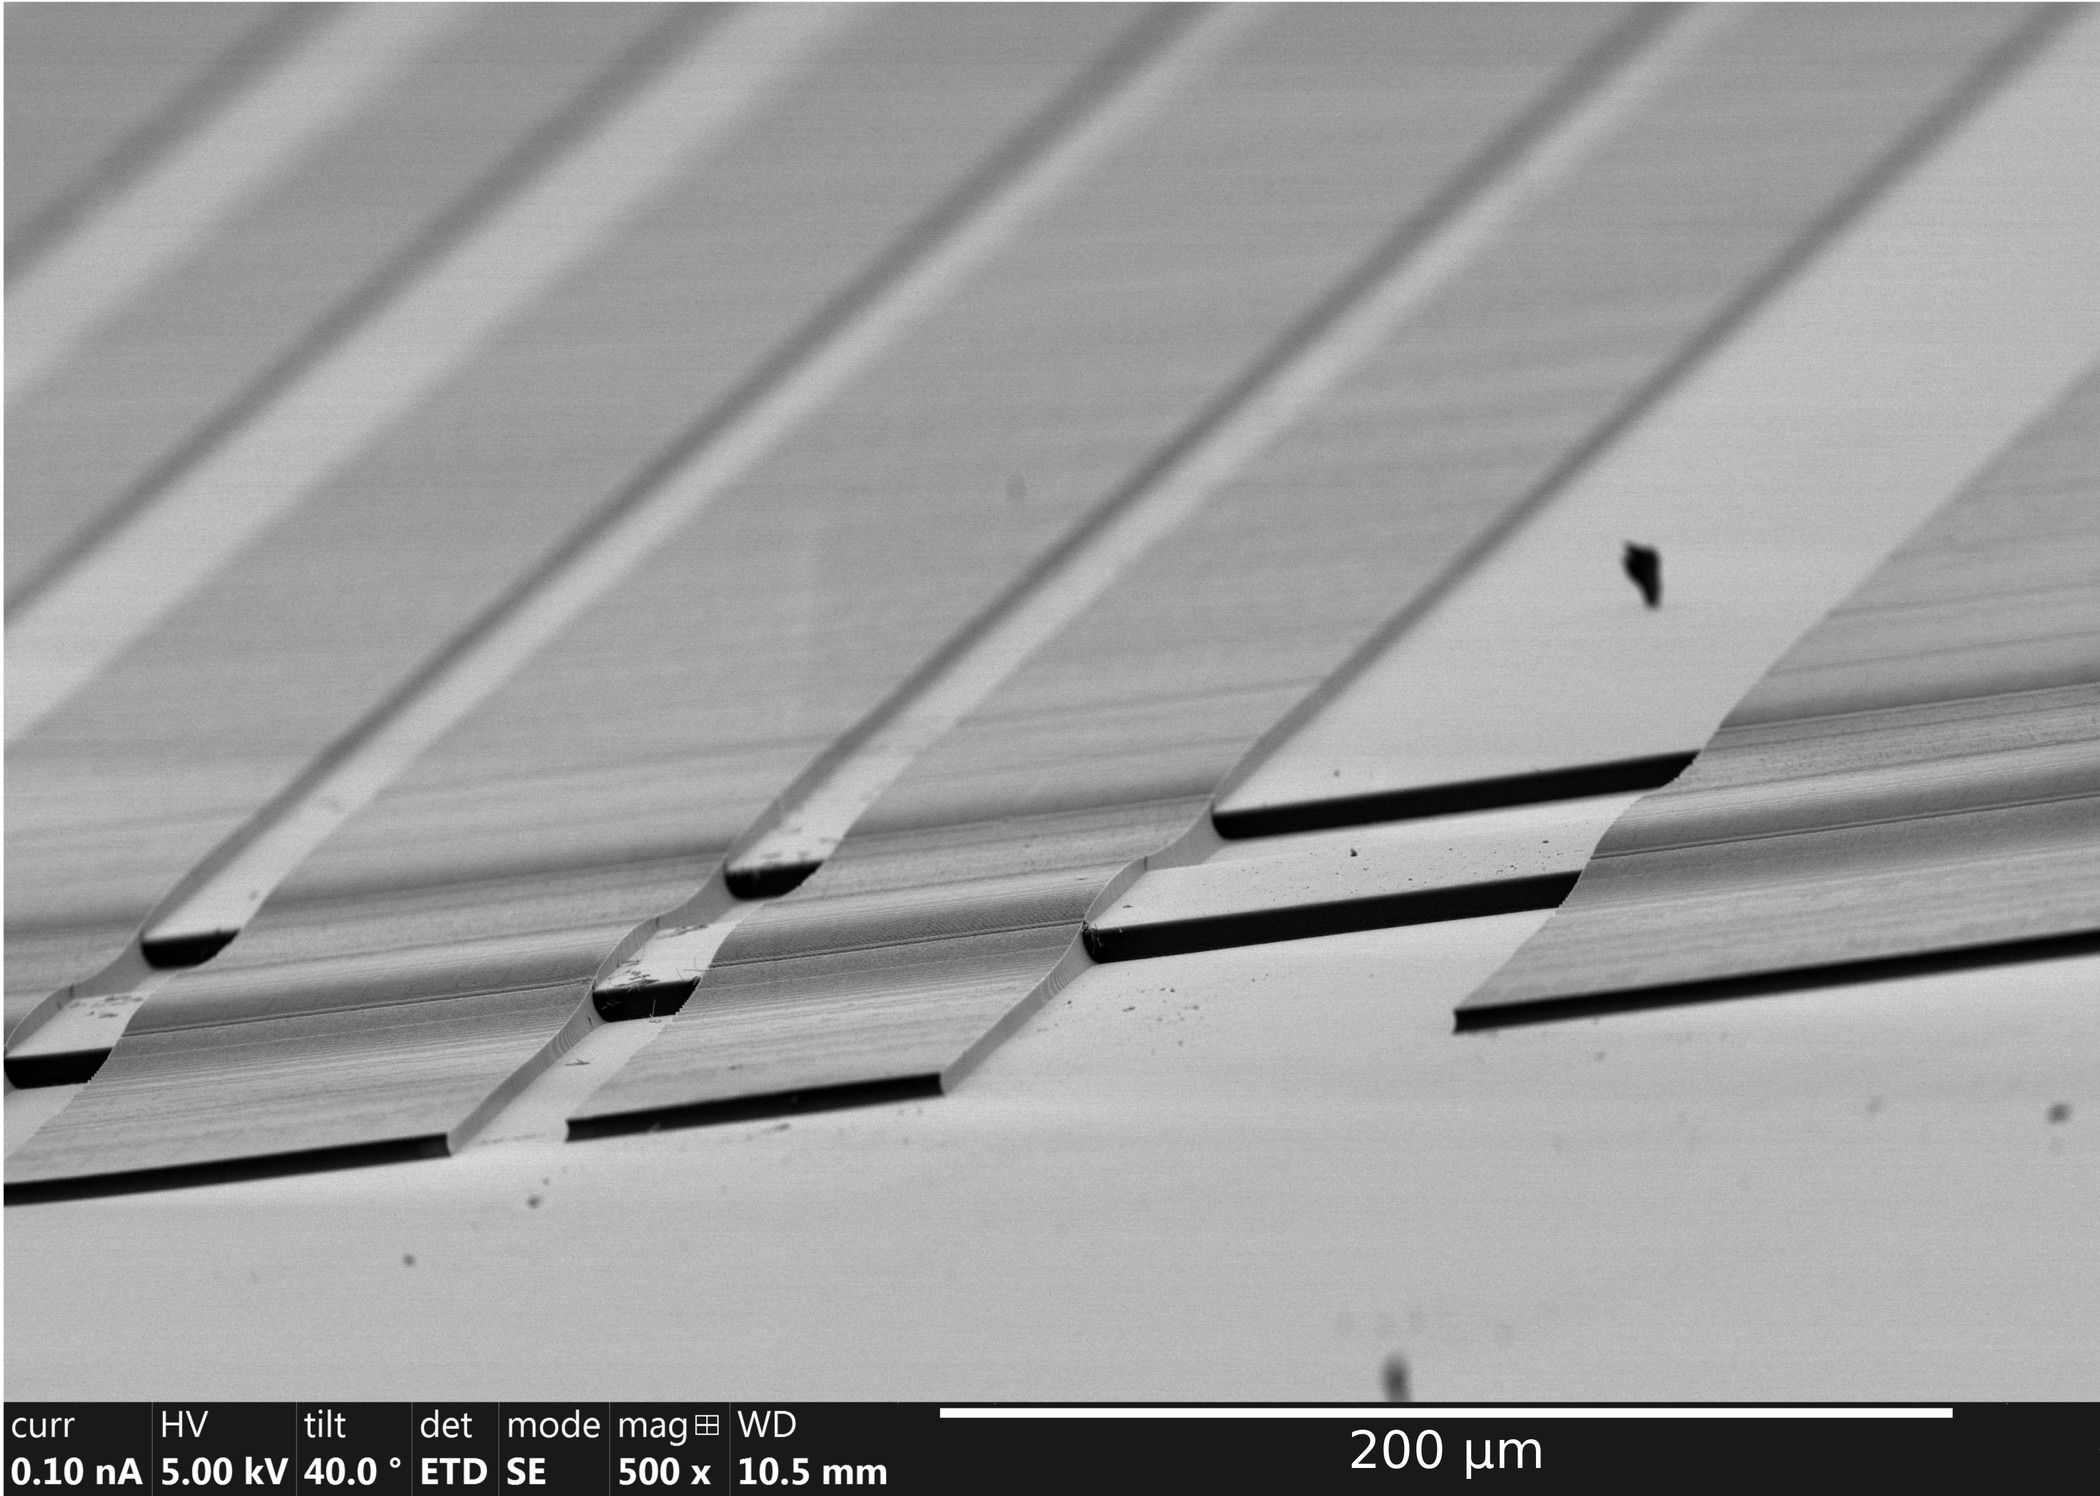
\includegraphics[width=\linewidth]{fig/mr-DWL/sem_mr-dwl-2.jpg}
  %\caption{1a}
  \label{fig:sfig1}
\end{subfigure}% %blank line makes figures vertical

\begin{subfigure}{.5\textwidth}
  \centering
  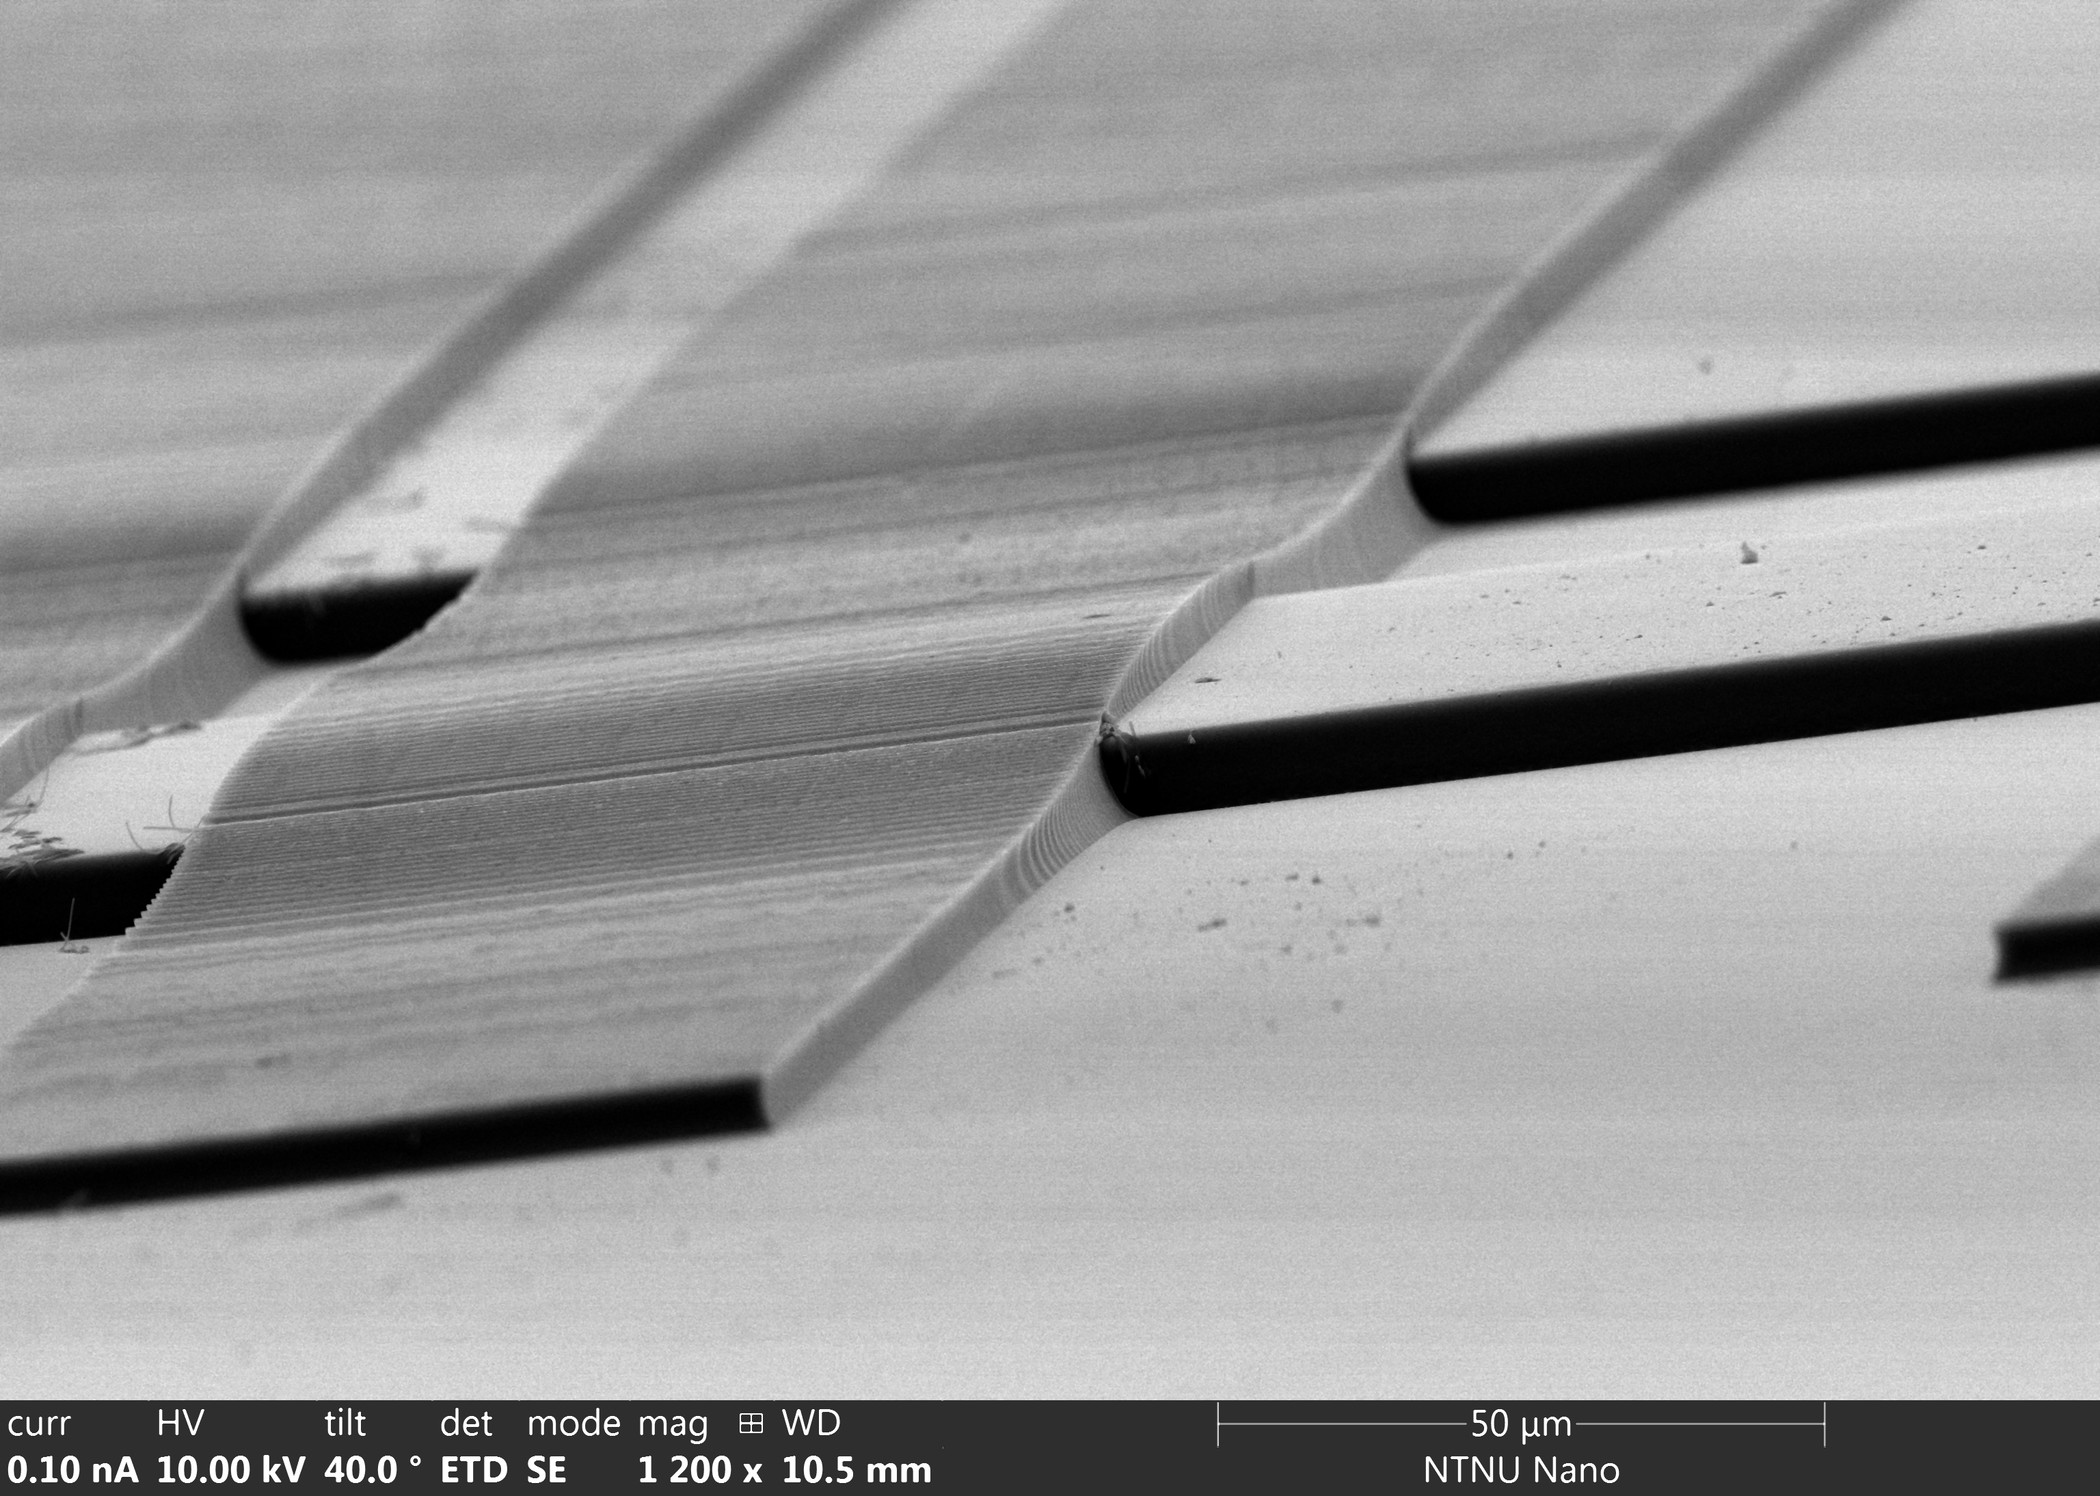
\includegraphics[width=\linewidth]{fig/mr-DWL/sem_mr-dwl.jpg}
  %\caption{1b}
  \label{fig:sfig2}
\end{subfigure}
\caption{$5um$ mr-DWL resist structures coated with a $4um$ man440 layer, demonstrating the possibility of patterning resist structures over a high step edge. }
\label{fig:fig}
\end{wrapfigure}

A remaining problem with the sample preparation is cracking in the glass cladding that impedes the path of the electrical contacts. This consistently happens in the form of a parallel crack propagating on at least one side of the core. Cracking becomes more severe in samples with a larger core to cladding ratio, and in hand drawn samples. Not only does this limit the contact spacing and the number of measurements that can be made on one sample, it also affects the ability to make hall measurements, as the hall pattern requires contacts on either side of the fiber. It is sometimes the case that only a small amount of a particular sample is drawn, and then each sample becomes more important, and a failure during preparation will set back the work significantly. Further if we desire to create structures or junctions within the fiber and characterize the core at the exact point the chances of cracking preventing measurement of the fiber are substantially higher. Due to the small size of the cracks, it is unlikely that filling them with a method such as vacuum impregnation with epoxy would be successful. Further this would require a second polishing step to remove this new layer from the core for electrical measurements.

While photoresist is mainly used for masking purposes, adding a permanent layer of resist would create a smooth surface and without coating the core, and has the advantage of integrating easily with the current process. A second lithography step would add little to the preparation time. The challenges are that the resist layer must be stable in solvent during a second liftoff process and that the contacts deposited over the resist, adhere well and can create continuous coverage of the resist step edge. For the latter a positive resist would be the ideal choice due to the positive sidewall profile. Further a greyscale resist such ma-p1275g  would allow thick films (~100 um) and a controllable positive sidewall profile. While ma-p1275G would be an ideal choice, tests showed that it was not significantly cross linked after hard baking to withstand an acetone bath. 

The negative photo resists $SU-8$ and $mr_DWL$ are epoxy based and designed for creating high aspect ratio structures with nearly vertical sidewalls. Further a hardbake step up to 140C creates a very stable resist. While the sidewall profile is still negative, tilting the sample during depostion, or using sputtering may allow sufficient step coverage to create a continuous contact. 

\section{Experimental Procedures}
A test sample using mr-DWL 5 was patterned on a Si wafer using the following parameters: spin 3000 rpm patterning $\SI{500}{\milli \joule \cm^{-2}}$ at $405 \si{\micro\meter}$ in the MLA, followed by a hard bake of 30 min $140 \si{\celsius}$. This structure was then coated with $\SI{4}{\micro \meter \cm^{-2}}$ man-440 using the standard recipe described above. 

The procedure was tested on a fiber to examine how the process would work under practical conditions, as the resist thickness, bake temperature and reflections during exposure would all be slightly effected. Electrical contacts were deposited using the standard recipe followed by a sputtered layer of $100 \si{\nano \meter}$. After electrical testing, a further layer of Au was deposited by sputter coating in a small cressington 208 HR B sputter coater, as this was the only method of deposition that allowed for tilting of the sample. Both test samples were analysed by 3d-optical profilometry and SEM. 

\section{MiBots}
An alternative to the Lithographic techniques described, is direct probing of the sample using micro manipulators. Imina Techinology Mibots are vacuum compatible micro manipulators with interchangeable tungsten probes capable of electrical probing. The probe positioning precision is in the nm range and is more than sufficient for fiber measurements. The MiBots have a stage that can be used with an optical or electron microscope. Use with an electron microscope allows for high accuracy in the measurement of the probe spacing. Direct probing has the advantage of eliminating the challenges associated with lithography, including the need to bridge an cracking in the glass fiber and any relief profile and possible chipping at the glass epoxy interface. Problems with metal adhesion to the three different materials (glass,epoxy,core) are substrate is also eliminated. While work has been done to use micromanipulators to characterize semiconductor fibers \cite{Engel2016DirectPhotosynthesis} past experience in our group has found that reliable electrical contact is difficult to achieve. %Ohmic contacts of the manipulators requires sufficient force (look up here). 
Depositing micro contacts along the core should provide a reliable method of contacting the sample while still avoiding many of the problems encountered with larger contacts.  



\begin{figure}[t]
  \centering
    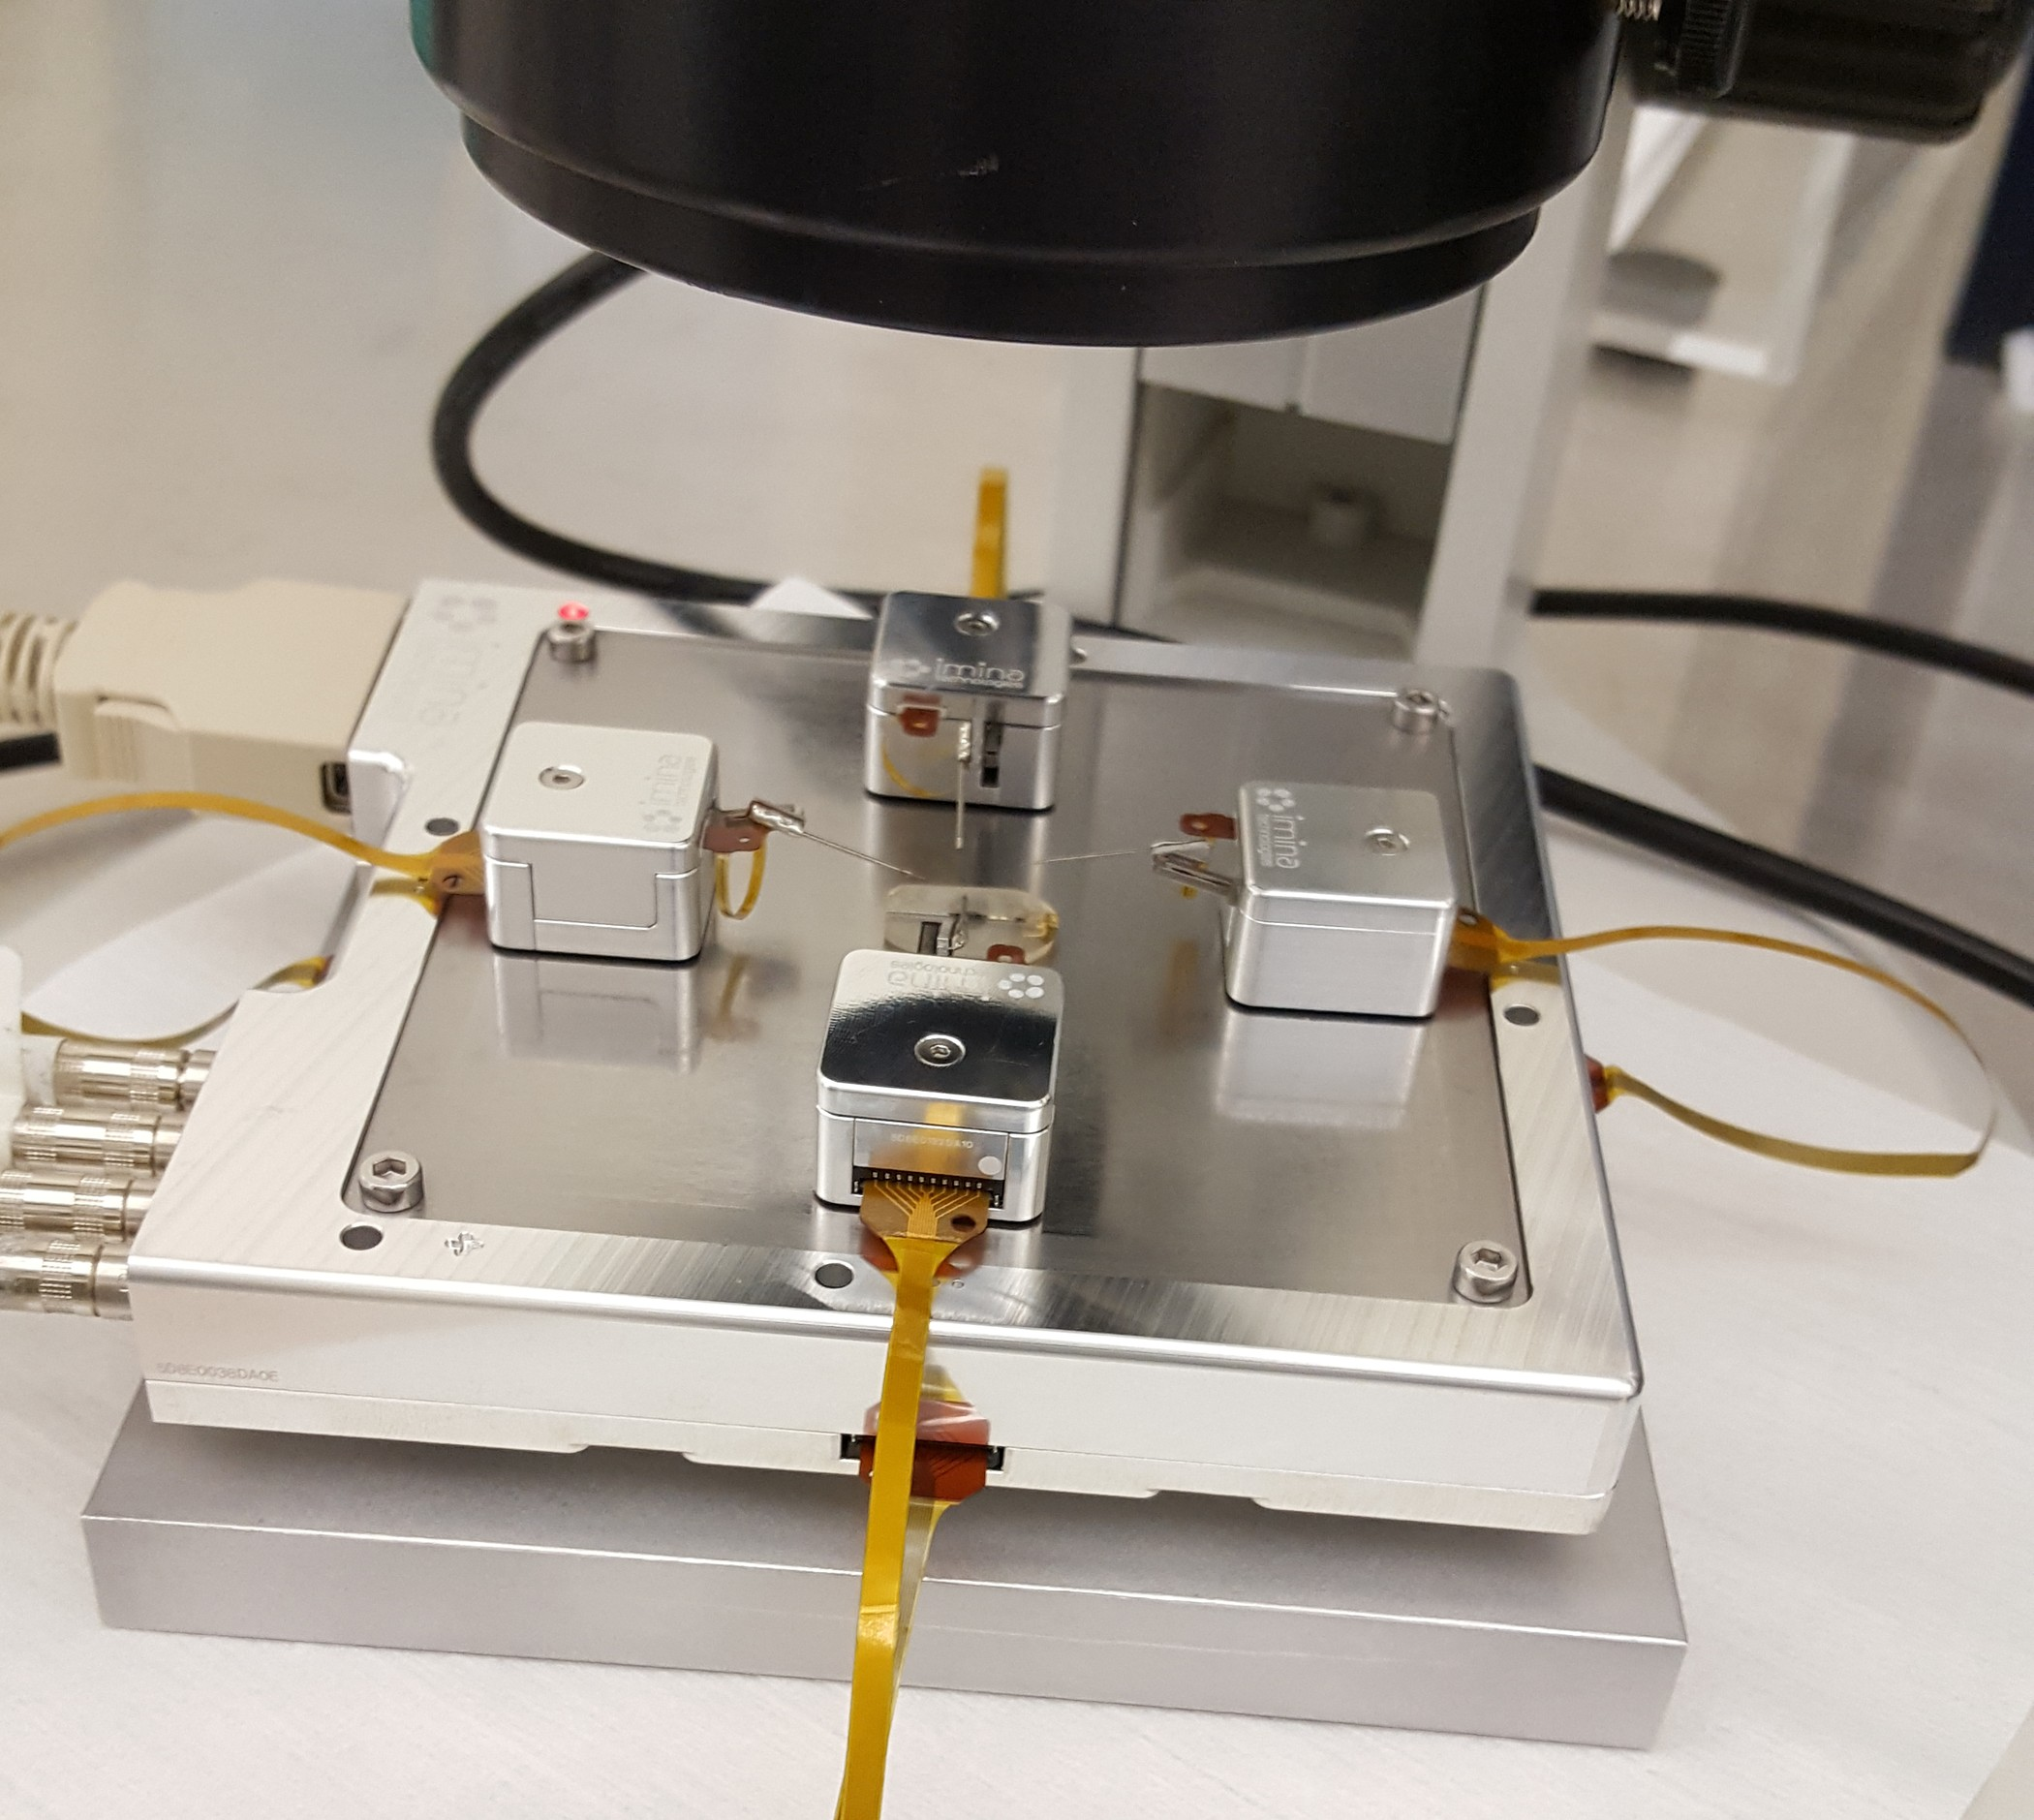
\includegraphics[width=0.7\textwidth]{fig/MiBots/setup.jpg}
 \caption{}
\label{mibot}
\end{figure}

\begin{figure}[t]
  \centering
    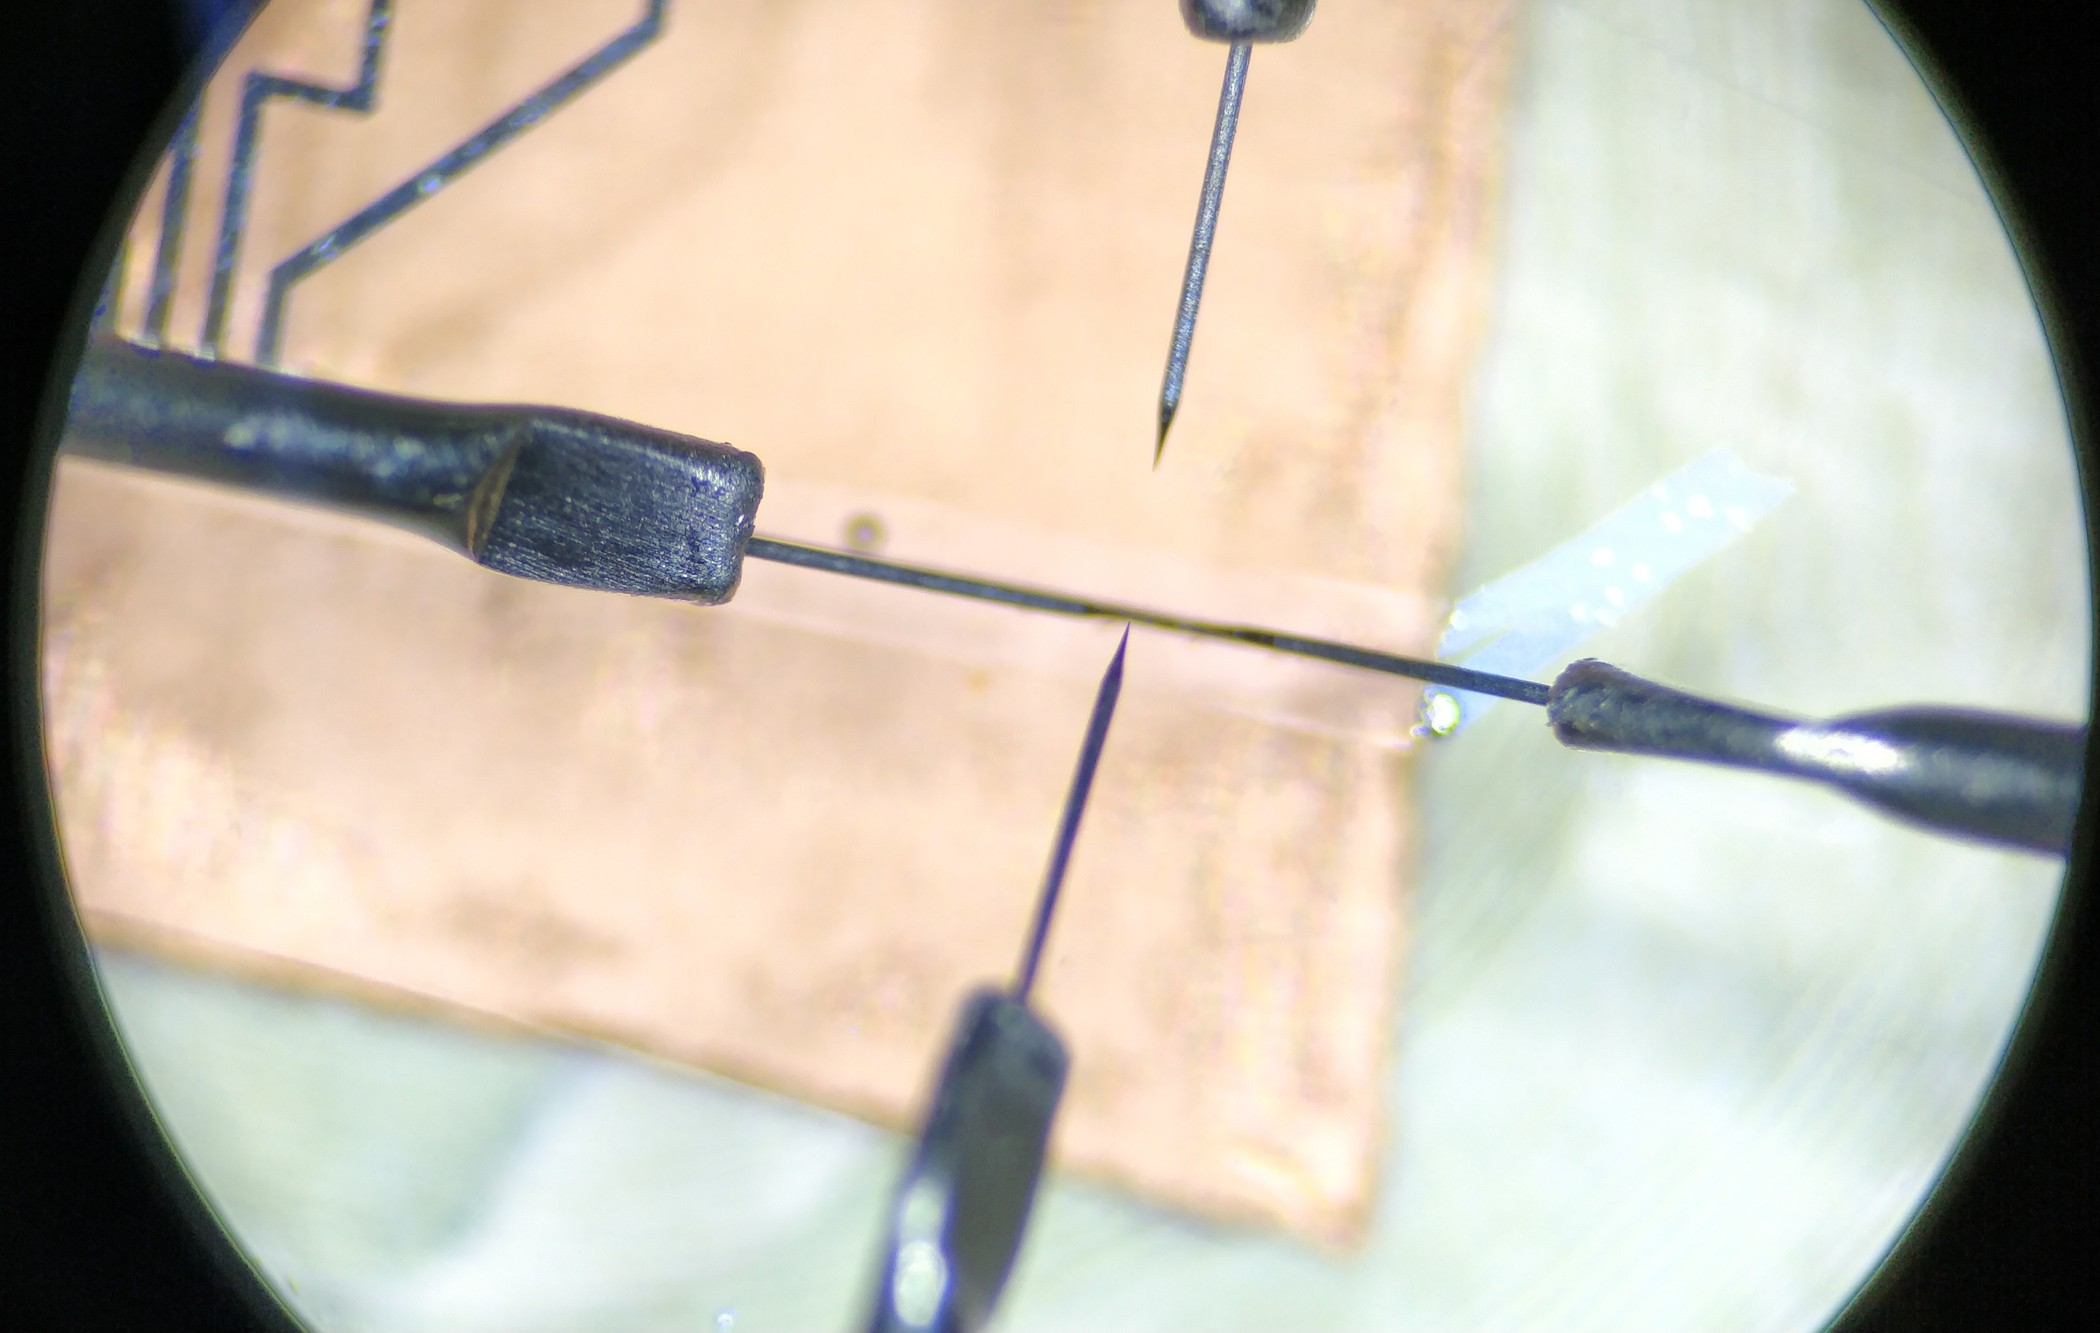
\includegraphics[width=0.7\textwidth]{fig/MiBots/IMG_20190409_143016.jpg}
 \caption{ Mibot with 1 um Probe tips directly contacting the exposed sample core. The two outer current carrying probes are in contact while the voltage probes are raised above the sample.}
\label{mibot}
\end{figure}

\begin{figure}[t]
  \centering
    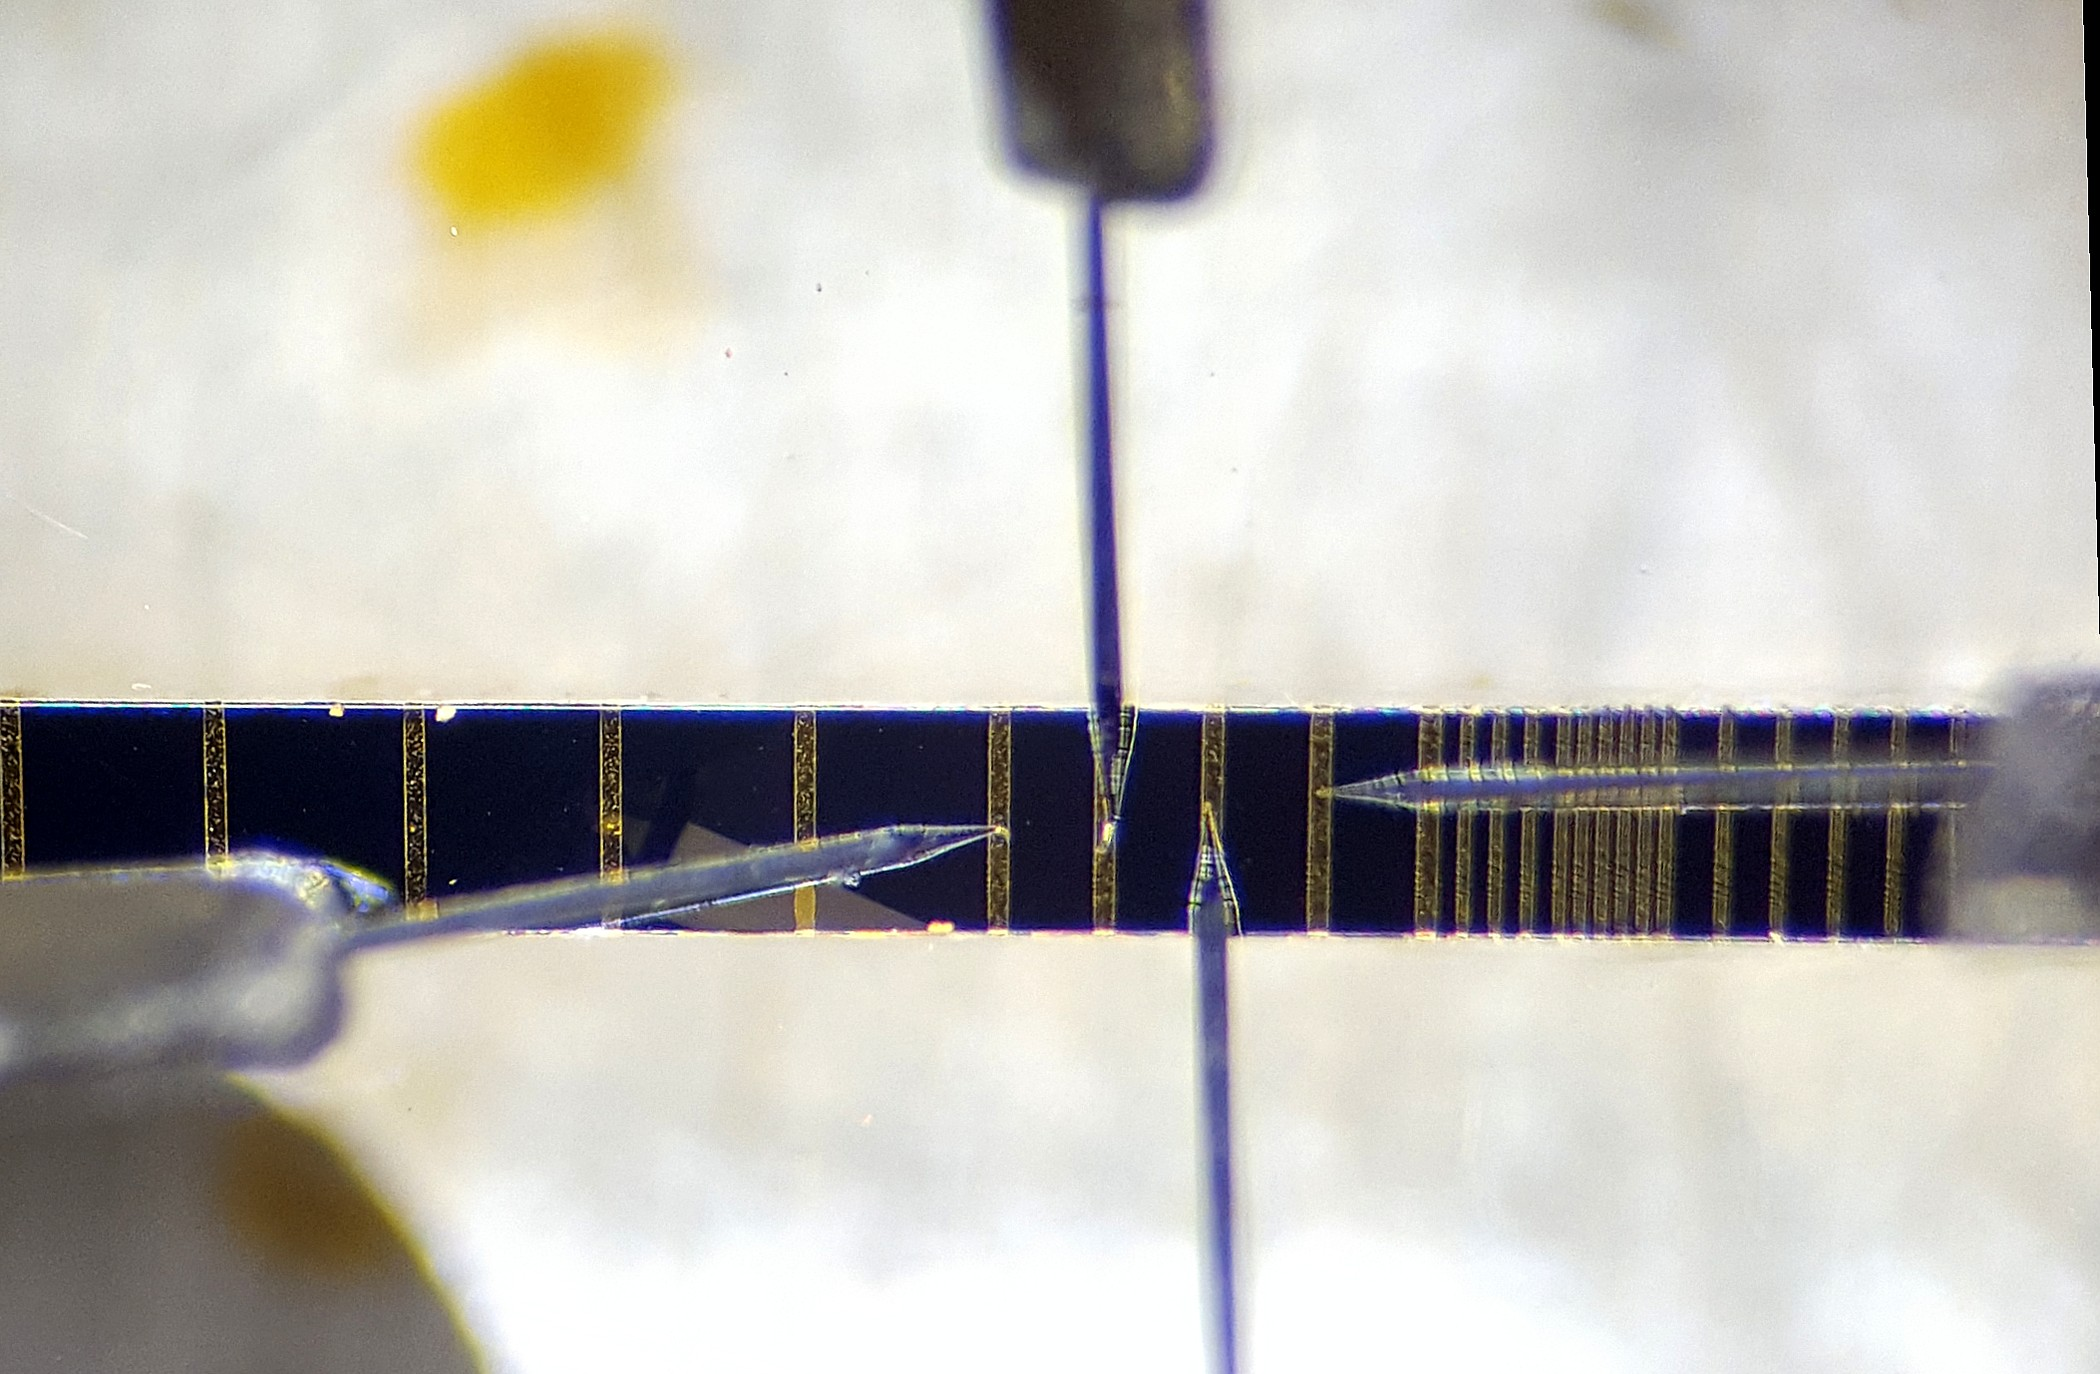
\includegraphics[width=0.7\textwidth]{fig/MiBots/closeup.jpg}
 \caption{}
\label{mibot}
\end{figure}

%\begin{fgure}[h]
%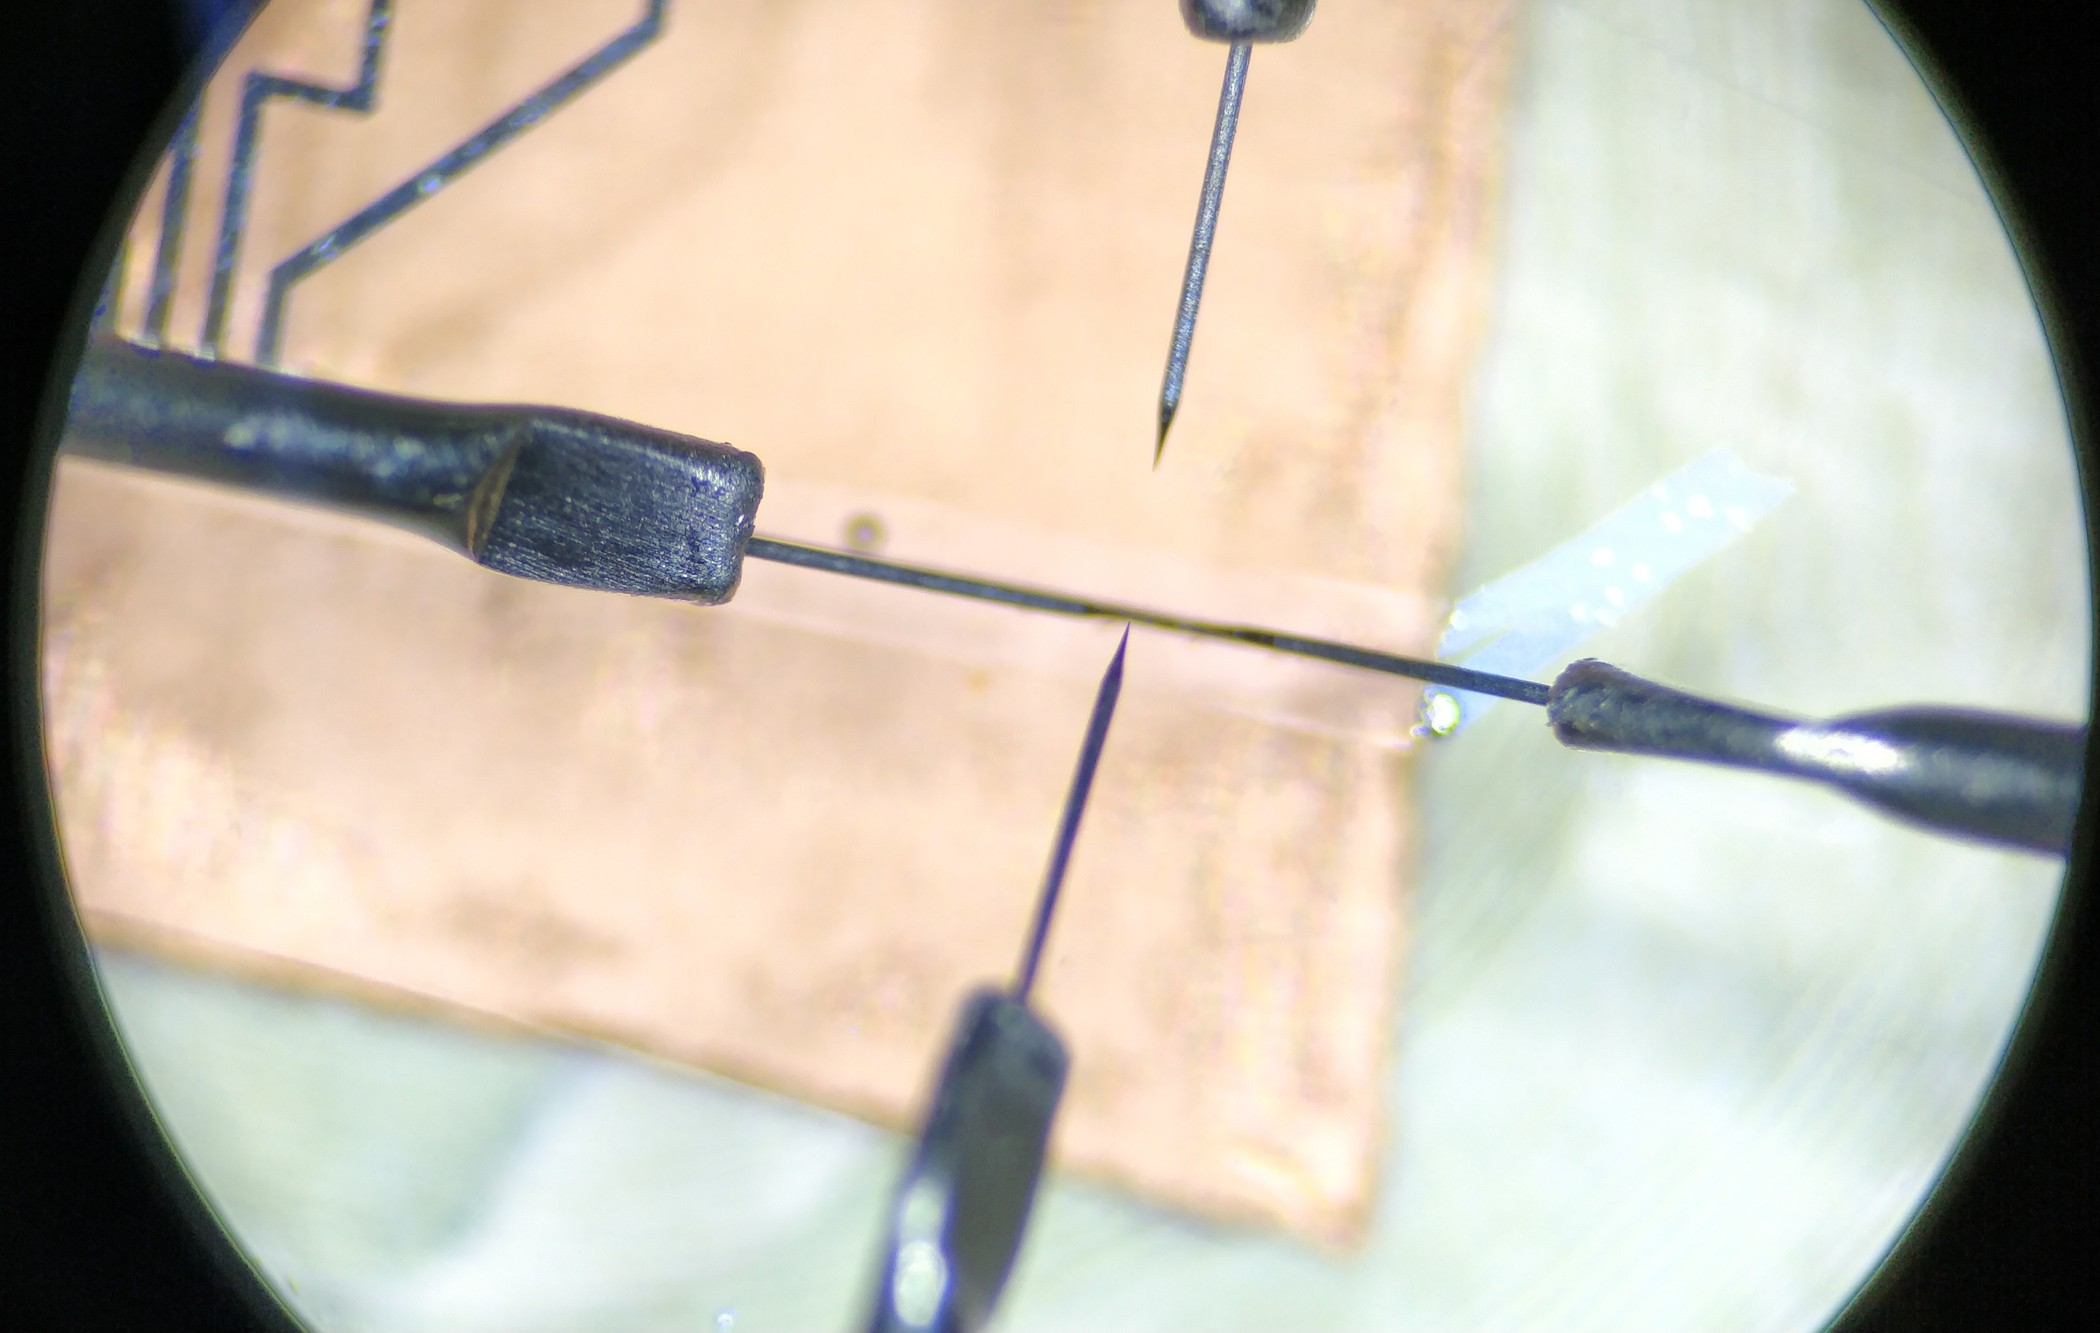
\includegraphics[width=.7\textwidth]{fig/MiBots/IMG_20190409_143016.jpg}
%\caption{Mibot with 1 um Probe tips directly contacting the exposed sample core. The two outer current carrying probes are in contact while the voltage probes are raised above the sample.}
%\end{figure}
\cleardoublepage